%  ========================================================================
%  Copyright (c) 1995-2012 The University of Washington
%
%  Licensed under the Apache License, Version 2.0 (the "License");
%  you may not use this file except in compliance with the License.
%  You may obtain a copy of the License at
%
%      http://www.apache.org/licenses/LICENSE-2.0
%
%  Unless required by applicable law or agreed to in writing, software
%  distributed under the License is distributed on an "AS IS" BASIS,
%  WITHOUT WARRANTIES OR CONDITIONS OF ANY KIND, either express or implied.
%  See the License for the specific language governing permissions and
%  limitations under the License.
%  ========================================================================
%

% Documentation for UW thesis document style for LaTeX
% by Jim Fox
% fox@washington.edu
%
%    Revised for version 2012/06/19 of uwthesis.cls
%
%    This document is contained in a single file ONLY because
%    I wanted to be able to distribute it easily.  A real thesis ought
%    to be contained on many files (e.g., one for each chapter, at least).
%
%    To help you identify the files and sections in this large file
%    I use the string '==========' to identify new files.
%
%    To help you ignore the unusual things I do with this sample document
%    I try to use the notation
%       
%    % --- sample stuff only -----
%    special stuff for my document, but you don't need it in your thesis
%    % --- end-of-sample-stuff ---


%    Printed in twoside style now that that's allowed
%

 % TODO: 11pt or 12?
\documentclass [12pt, oneside] {uwthesis}[2012/06/19]
 
%
% The following line would print the thesis in a postscript font 

% \usepackage{natbib}
% \def\bibpreamble{\protect\addcontentsline{toc}{chapter}{Bibliography}}

\setcounter{tocdepth}{1}  % Print the chapter and sections to the toc
 

% ==========   Local defs and mods
%

% --- sample stuff only -----
% These format the sample code in this document

\usepackage{alltt}  % 
\newenvironment{demo}
  {\begin{alltt}\leftskip3em
     \def\\{\ttfamily\char`\\}%
     \def\{{\ttfamily\char`\{}%
     \def\}{\ttfamily\char`\}}}
  {\end{alltt}}
 
% metafont font.  If logo not available, use the second form
%
% \font\mffont=logosl10 scaled\magstep1
\let\mffont=\sf
% --- end-of-sample-stuff ---
 
% Math stuff
\usepackage{amsmath}
\usepackage{hyperref}
\usepackage{graphicx}
\usepackage{float}
\usepackage{tabularx}

\setlength{\intextsep}{5pt}           % Controls spacing around float environments

\begin{document}
 
% ==========   Preliminary pages
%
% ( revised 2012 for electronic submission )
%

\prelimpages
 
%
% ----- copyright and title pages
%
\Title{Programmable System for Laser Control of Trapped-Ion Experiment}
\Author{Haochen Yu}
\Year{2025}
\Program{Electrical and Computer Engineering  }

\Chair{Scott Hauck}{}{Department of Electrical and Computer Engineering}
\Signature{Sara Mouradian }


\copyrightpage

% \titlepage  

% --- sample stuff only -----
% unusual footnote not found in a real thesis
% You just use the \titlepage as commented out above

{\Degreetext{A thesis%
  submitted in partial fulfillment of the\\ requirements for the degree of}
 \let\footnoterule\relax
 \titlepage
 }
\setcounter{footnote}{0}

% --- end-of-sample-stuff ---
 
%
% ----- signature and quoteslip are gone
%

%
% ----- abstract
%


\setcounter{page}{-1}
\abstract{%
This sample dissertation is an aid to students who are attempting
to format their theses with \LaTeX, a sophisticated
text formatter widely available at the University of Washington
and other institutions of higher learning.
 

}
 
%
% ----- contents & etc.
%
\tableofcontents
\listoffigures
\listoftables 
 
%
% ----- acknowledgments
%
\acknowledgments{% \vskip2pc
  % {\narrower\noindent
 
  % \par}
}
 
 
 
%
% ==========      Text pages
%

\textpages


\chapter{Introduction}

Trapped-ion quantum computing stands at the forefront of modern quantum technology, promising unparalleled computational capabilities through the manipulation of individual atomic ions. A cornerstone of these systems is the laser control unit, which must deliver precisely tailored optical pulses with extreme timing accuracy \cite{manychanfpgactrlsys}. Motivated by recent advances in both quantum experiments and control hardware, this thesis presents a novel laser control system specifically designed for trapped-ion quantum computing.

This hardware design, implemented on a Xilinx Zynq FPGA platform, harnesses the combined power of high-speed and low-speed digital-to-analog converters (DACs) to achieve synchronous control across 32 discrete laser channels. With a frequency of 100 MHz, the system meets the rigorous temporal precision required for high-fidelity qubit manipulation. Such demanding performance is essential, as even slight deviations in timing can significantly impact the accuracy and repeatability of quantum operations \cite{manychanfpgactrlsys}.

The design approach is both well-structured and modular, ensuring a robust foundation for development. Initially, a single pulse channel is developed and rigorously evaluated as a proof-of-concept. This initial validation is crucial as it demonstrates the feasibility and effectiveness of the design. Once the single channel is successfully validated, it is scaled into a comprehensive system by integrating custom programmable logic blocks. These blocks are designed to efficiently deliver stable DC voltage control and generate dynamic, high-frequency pulsed waveforms. This capability ensures versatile and precise signal manipulation. The scalability and modularity of the design not only meet current experimental demands but also provide a robust framework that can adapt to future challenges in quantum computing \cite{programmablesoc4ctrlexperiment}. This adaptability is particularly important as it allows the system to evolve with advancements in the field, ensuring long-term relevance and utility.

Central to the system's performance is its effective exploitation of the FPGA's built-in features. By incorporating custom memory IP, high-speed internal communication interfaces, and an embedded ARM CPU core, the design achieves remarkable throughput and robustness. This careful coordination of resources ensures precise hardware timing and optimal utilization. This strategic use of FPGA capabilities underscores the system's ability to deliver high performance and reliability.
\chapter{Background}

\section{Laser Trapped-Ion Experiment}

Trapped-ion quantum systems have emerged as a leading candidate for quantum computing platforms due to their exceptional coherence times, high-fidelity quantum gates, and promising scalability. In trapped-ion systems, ions—charged atoms confined by electric fields—are precisely controlled and manipulated using laser beams. These lasers serve critical roles, including initializing quantum states, implementing quantum gates, and performing state measurements \cite{naturequantuminfo}. These lasers serve critical roles, including initializing quantum states, implementing quantum gates, and performing state measurements.

However, traditional approaches for optical hardware tend to be bulky, expensive, and power-intensive, posing severe limitations on scalability. As the number of qubits in a trapped-ion quantum computing system grows, these challenges become more pronounced \cite{photonicreview}. Compact, efficient, and rapid modulation capabilities are thus essential to scale quantum computing platforms beyond small-scale demonstrations.

Recent advancements in photonic integrated circuits (PICs) have substantially addressed these challenges \cite{apic}. These PICs are miniaturized, enabling direct integration with ion-trap chips, thereby dramatically reducing optical losses, system complexity, and the overall footprint. Crucially, integrated modulators facilitate modulation at very high speeds—on the order of nanoseconds—which matches the stringent timing requirements of quantum operations \cite{naturequantuminfo}.

To fully utilize the capabilities of these advanced PICs, corresponding electronic control systems capable of generating precisely timed, flexible modulation signals at around 100 MHz resolution are necessary. The 100 MHz resolution provided by the system ensures that the modulation signals can be precisely timed and shaped, directly corresponding to the stringent timing requirements of quantum gates that often operate on microsecond timescales. Having 32 synchronous dynamic voltage channels is essential because it allows the simultaneous manipulation of multiple qubits with coherent precision. The precise synchronization of these channels ensures minimal timing jitter and improved gate fidelity, which is indispensable for scaling quantum computing systems \cite{manychanfpgactrlsys}.

\section{Hardware Description}

To meet the demands of advanced control electronics, this project utilizes a Field Programmable Gate Array (FPGA). FPGAs excel at high-speed, low-latency parallel processing, enabling the simultaneous control of multiple channels and the implementation of flexible, efficient digital signal processing algorithms. These capabilities make FPGAs particularly suited for managing complex experimental setups that demand precise timing and real-time adaptability. This project employs the Xilinx Zynq UltraScale+ ZCU102 Evaluation Board, a robust platform chosen for its exceptional computational resources and flexible high-speed interfacing capabilities.

The ZCU102 board is integral for generating precise modulation signals required by quantum lasers. It features a range of peripherals, including PMOD interfaces that support low-speed digital-to-analog converters (DACs) via SPI protocols, and two FMC HPC connectors for high-speed DACs, essential for waveform generation. The core of this FPGA platform is the Xilinx Zynq architecture, which seamlessly combines a Processing System (PS) with Programmable Logic (PL) \cite{XilinxUG1182}.

The PS is powered by a quad-core Arm\textsuperscript{\textregistered} Cortex\textsuperscript{\textregistered}-A53 processor, capable of running real-time processing applications. It incorporates multiple peripherals, such as DDR4 memory for application storage and an Advanced eXtensible Interface (AXI) that connects the PS to other components, including the programmable logic. The PL, essentially the FPGA itself, is equipped with essential resources such as logic cells, flip-flops, and block RAMs (BRAM) \cite{XilinxUG1182}. It provides ample capacity for storing intermediate data.

This project leverages programmable logic to build custom hardware designs that serve the unique demands of quantum laser experiments. The FPGA's dedicated logic circuits and integrated high-speed interfaces enable quick, reliable communication with external modules. This capability is crucial for maintaining accurate control and precise timin. General-purpose I/O options, such as PMOD and FMC connectors, further simplify the experimental setup. These connectors offer flexible interfacing, allowing for both low-speed and high-speed connections that scale to the experiment's complexity without sacrificing performance.

In addition to the hardware features, a Python interface abstracts the low-level hardware details, streamlines testing and integration with the FPGA platform. Behind the scenes, a custom C-based program running in the processing system translates data from the Python interface into a format that the FPGA can efficiently process. This layered approach bridges high-level control with low-level hardware performance, ensuring that experimental algorithms and rapid prototyping can be achieved with reliability and precision.

\section{Pulse Sequence}

In high-fidelity quantum computing and atomic manipulation, pulsed sequences are essential for delivering precise, accurate, and stable outputs to photonic integrated circuits \cite{apic}. These laser pulses depicted in \autoref{fig:pulse_seq} are designed with a controlled shape that consists of three distinct phases: rise, sustain, and fall. Each phase plays a vital role in ensuring that quantum operations are performed reliably.

\begin{figure}[h]
    \centering
    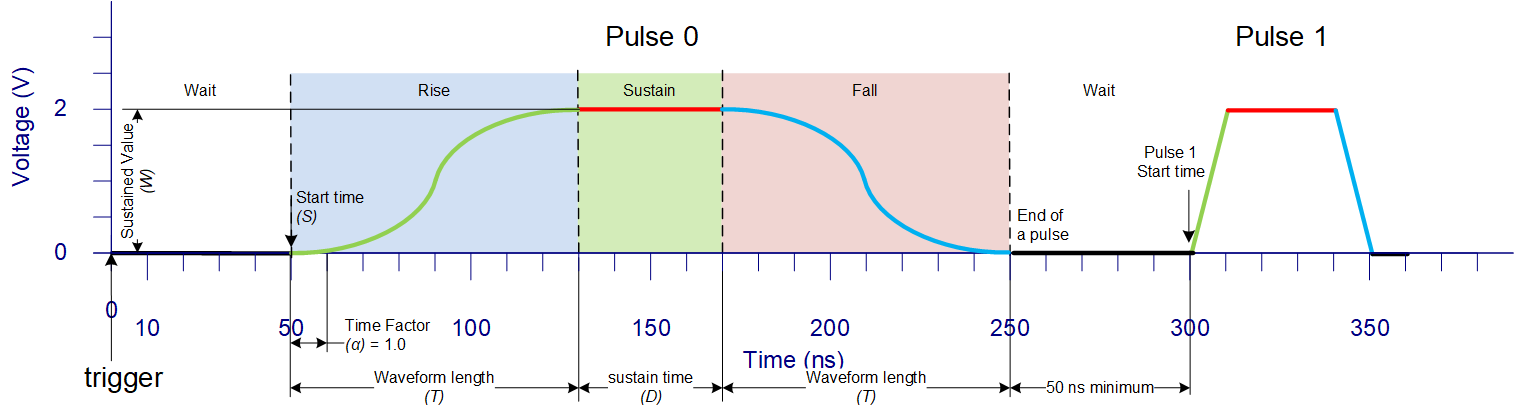
\includegraphics[width=1\linewidth]{figures/2.1.png}
    \caption{Waveform shape of the pulse sequence.}
    \label{fig:pulse_seq}
\end{figure}

During the rise phase, the laser intensity increases to its target level. A well-controlled rise minimizes errors and ensures that the experiment operate exactly when needed. The sustain phase follows, during which the laser maintains a constant optical intensity. This steady state is crucial because any fluctuation can compromise the fidelity of quantum gates by introducing operational errors \cite{naturequantuminfo}. Finally, the fall phase allows the laser power to decrease smoothly. Notably, maintaining symmetry between the rise and fall phases is critical for consistency and repeatability. In this design, the fall essentially becomes the reciprocal of the rise.

The waveform is generated as a series of discrete values representing a continuous function, with samples taken every 10 nanoseconds by the digital-to-analog converter (DAC). These sample values can be adjusted from a set of parameters to fine-tune the laser's output. For a waveform $f(x)$, a pulse $g(x)$ generated by the hardware to the laser can be defined by:

\begin{equation}
g(x) = A \cdot 
\begin{cases} 
f\left(\dfrac{\alpha(x - S)}{T}\right), & \!\!\! S \leq x < S + \left\lceil \frac{T-1}{\alpha} \right\rceil, \\[8pt]
f\left(\dfrac{T-1}{T}\right), & \!\!\! S + \left\lceil \frac{T-1}{\alpha} \right\rceil \leq x < S + \left\lceil \frac{T-1}{\alpha} \right\rceil + D, \\[8pt]
f\left(\dfrac{\alpha\left(2\left\lceil \frac{T-1}{\alpha} \right\rceil + D - (x - S) - 1\right)}{T}\right), & \!\!\! S + \left\lceil \frac{T-1}{\alpha} \right\rceil + D \leq x < S + 2\left\lceil \frac{T-1}{\alpha} \right\rceil + D - 1, \\[8pt]
0, & \!\!\! \text{otherwise}.
\end{cases}
\end{equation}



where $S$ is the pulse start time, $T$ is the waveform rise's length, $\alpha$ is the time factor, $D$ is the sustain time, and $A$ is the gain factor.
\chapter{Block Architecture}

\section{Functional Specification}

The pulse channel module generates precisely timed laser pulses using user-defined configurations, base waveforms, and a fixed sequence length. It relies on Xilinx block RAM IPs, a robust state machine, and versatile interfaces to produce a 16-bit waveform for an external 16-bit DAC.

Each pulse has symmetrical rise and fall edges, so the design only stores the rising edge data in one memory block. This decision reduces memory usage and simplifies the waveform generation process by eliminating redundant information. Another RAM block holds the complete waveform definition, including critical details such as start times. This separation allows for dynamic updates to the base shape without altering existing data. The benefit of this approach is that it minimizes resource usage and makes real-time adjustments easier.

The pulse generator is activated by an external trigger, ensuring that the system is both flexible and responsive. Once triggered, the module reads the RAM-stored configuration, processes the waveform through the state machine, and outputs the corresponding pulse. Multiple waveform variations can be defined, allowing the system to seamlessly transition from one pulse definition to the next until the entire sequence is completed. The resulting 16-bit waveform is then transmitted through the FPGA's AXI-stream interface to the external DAC. Standard signaling protocols such as valid, ready, and last manage data transfer and synchronization, ensuring that the pulse shape is preserved with minimal latency.

All waveform data and parameters are loaded into RAM via a 32-bit data, 12-bit address interface. This interface supports both configuration and monitoring, enabling the module to select between the RAM blocks or perform real-time diagnostics and debugging. This flexibility allows for rapid reconfiguration and continuous system oversight, which is essential for maintaining its high performance.

Error handling is integrated into the module. Dedicated error signals are generated during pulse generation to detect anomalies and trigger immediate responses. Pipeline delays are carefully managed to ensure signal synchronization and maintain timing margins across the data path.

\begin{figure}[h]
    \centering
    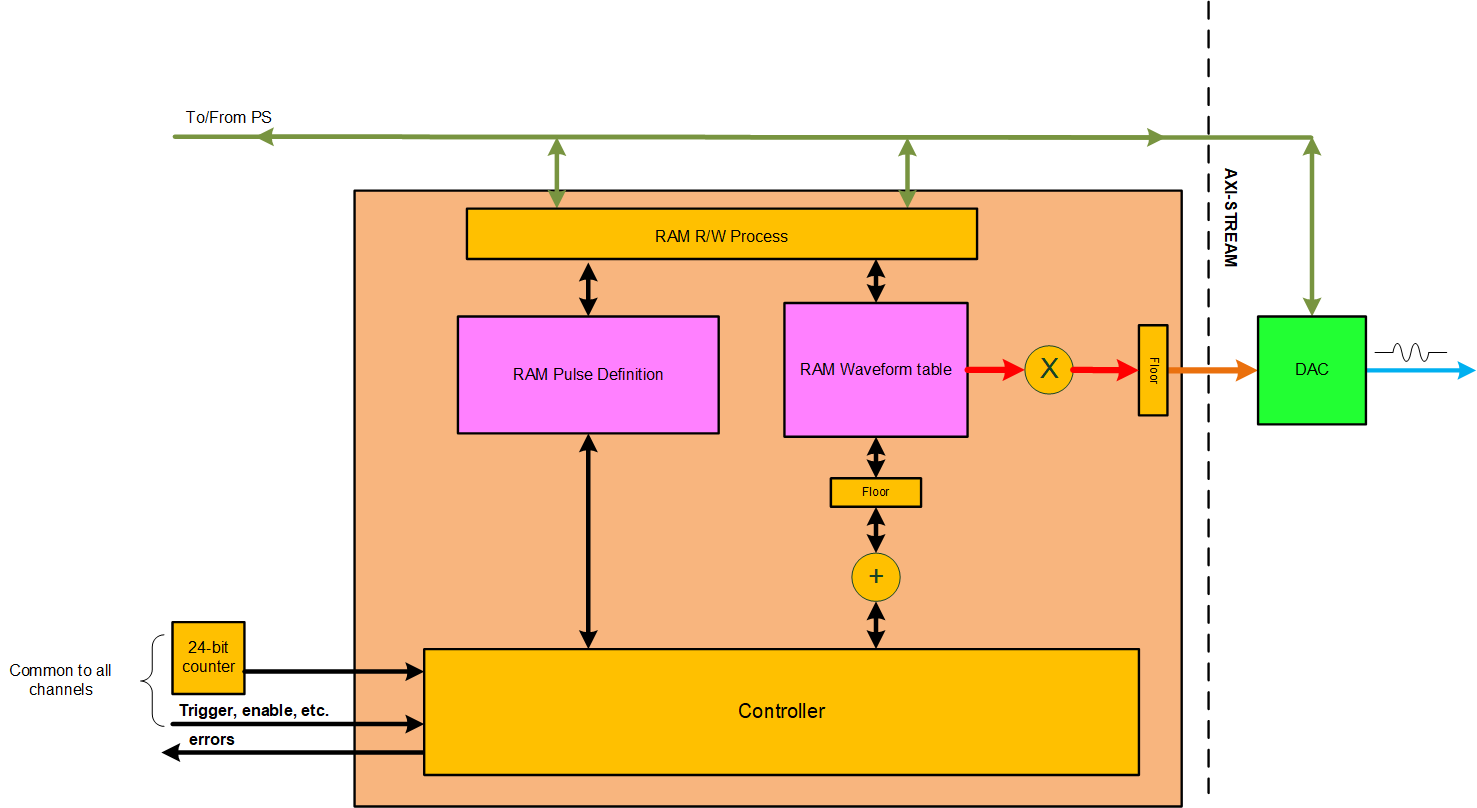
\includegraphics[width=1.0\linewidth]{figures/3.1.png}
    \caption{Block diagram of the pulse channel with two RAMs integrated.}
    \label{fig:block_diagram}
\end{figure}

\section{Setup}

The pulse channel module uses two dual-port memories with Xilinx Block Memory Generator \cite{blockmemgen}, as shown in \autoref{fig:block_diagram}. This design choice allows for dynamic waveform generation with configurable parameters, ensuring system responsiveness through parallel access. One port of each memory is read-only, dedicated to the internal controller for waveform generation. The other port is read-write, enabling data to be loaded and stored efficiently. This setup optimizes memory usage and enhances the module's flexibility and performance.

\subsection{Memory Organization and structure}

The module uses two block memories, each serving a unique purpose for high-speed waveform generation. The pulse definition (PD) memory is a 1024x32-bit dual-port block RAM that stores comprehensive waveform parameters. This allows for reconfiguring waveforms in multiple forms without needing to change data in the hardware. The waveform data is stored in the dual-port 4096x16-bit waveform table (WT) memory. This memory holds the base form of the rising edge of the waveform.

The dual-port configuration of both memories is a critical architectural decision, enabling concurrent access from both external interfaces and internal controls for waveform generation. This parallelism ensures that ongoing pulse generation operations remain unaffected by system configuration updates.

\subsection{Pulse Definition}

\begin{figure}[htbp]
    \centering
    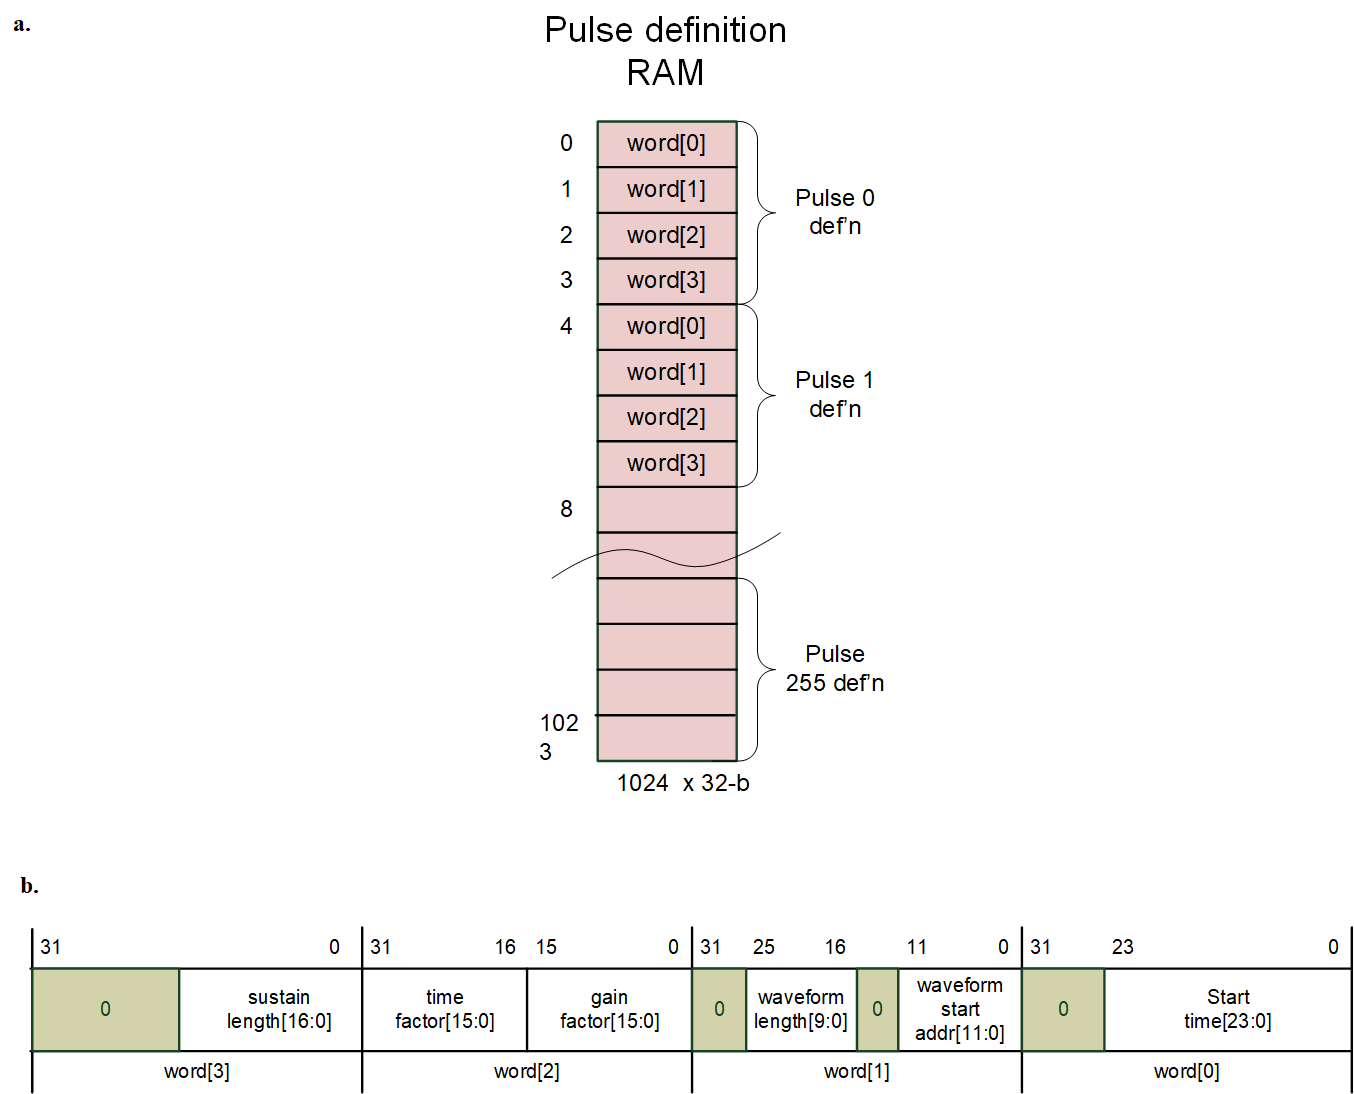
\includegraphics[width=1\linewidth]{figures/3.2.png}
    \caption{\centering{Pulse Definition RAM overall allocation. \textbf{a}, the overall allocation in the memory. \textbf{b}, specific bit-wise allocations of each pulse’s parameter.}}
    \label{fig:pd}
\end{figure}

The pulse definition memory employs a well-organized addressing scheme, where each set of pulse parameters is allocated four consecutive 32-bit memory locations. This means that the parameters for each pulse are stored sequentially, as illustrated in \autoref{fig:pd}a. In other words, each pulse parameter set is 128 bits in length, occupying four consecutive byte addresses. Consequently, the 1024-address memory can accommodate up to 256 pulses per channel, allowing for either unique pulses or variations based on another. This structured approach ensures efficient storage and retrieval of pulse parameters. By organizing the memory in this manner, the system can handle a significant number of pulses while maintaining clarity and ease of access. Each pulse's parameter is defined by \autoref{fig:pd}b and \autoref{tab:pd_param}.

\begin{table}[htbp]
    \centering
    \begin{tabularx}{\textwidth}{|c|X|X|}
        \hline
        Word \# & Name & Description \\
        \hline
        0 & Start Time & Time a pulse should start \\
        \hline
        1 & Waveform Start Address & Starting address of the waveform table memory \\
        \hline
        1 & Gain Factor & Scale the amplitude of the output signal. Within (0,1] \\
        \hline
        2 & Time Factor & Step Size adjusts the rate at which the pulse's rise or fall is executed. In the range [1, waveform length) \\
        \hline
        2 & Waveform Length & Duration of the rise (when the time factor is one). \\
        \hline
        3 & Sustain Length & Duration in 10ns scale of last wave value after rise stage should stay before start the fall stage \\
        \hline
    \end{tabularx}
    \caption{Detailed pulse's parameter set}
    \label{tab:pd_param}
\end{table}



\subsection{Waveform Table}
The waveform table memory is designed to store the base values for the rise of each pulse. As shown in \autoref{fig:wavetable}, each entry in the table consists of a pair of 16-bit values. This design is necessary because at least two values are required to construct the rise or fall of a pulse. A pulse's rise can store up to 2048 32-bit value pairs, or 4096 16-bit data points, in the waveform table memory. The number of value pairs used for each pulse depends on its waveform length. If the waveform length is even, it takes half of the waveform length in value pairs. If the length is odd, it takes the floor of the waveform length divided by 2, plus the lower value of the next pair.
\begin{figure}[htbp]
    \centering
    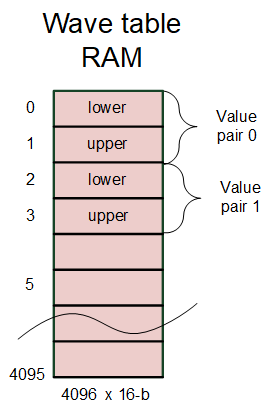
\includegraphics[width=0.30\linewidth]{figures/3.3.png}
    \caption{Memory layout for waveform table}
    \label{fig:wavetable}
\end{figure}
The memory allocation in the waveform table is dynamic, relying on waveform lengths and start addresses from the pulse definition. This design is purpose-built to maximize memory utilization. By adapting the allocated space based on each pulse's requirements, the system can store a single pulse with a maximum length of 4096 data points, or distribute storage among up to 256 pulses where each pulse uses no more than 16 data points on average. This approach ensures that longer pulses receive the space they need while shorter pulses occupy only what is necessary, thus avoiding wasted memory and maintaining efficient resource use.

Furthermore, the waveform table allows multiple pulse definition points to reference the same memory region, given that their start addresses and waveform lengths are identical. This capability is especially beneficial when different scale factors are applied to the same pulse structure. By sharing the memory region, the design avoids redundant storage of waveform data and minimizes additional space usage. 

\section{Procedure}
The module creates precise pulse-shaped waveforms by progressing through a series of well-defined states, shown in \autoref{fig:fsm}. It activates when an external trigger is received from the system while the module is enabled, shown in the bottom left of \autoref{fig:block_diagram}. Upon receiving the trigger, the module loads the necessary data from the pulse definition memory into a set of registers. It then enters a waiting stage and holds until a 24-bit timer reaches the predetermined start time. This approach guarantees that each pulse is generated precisely when needed—a key requirement for synchronization in FPGA applications.
\begin{figure}[htbp]
    \centering
    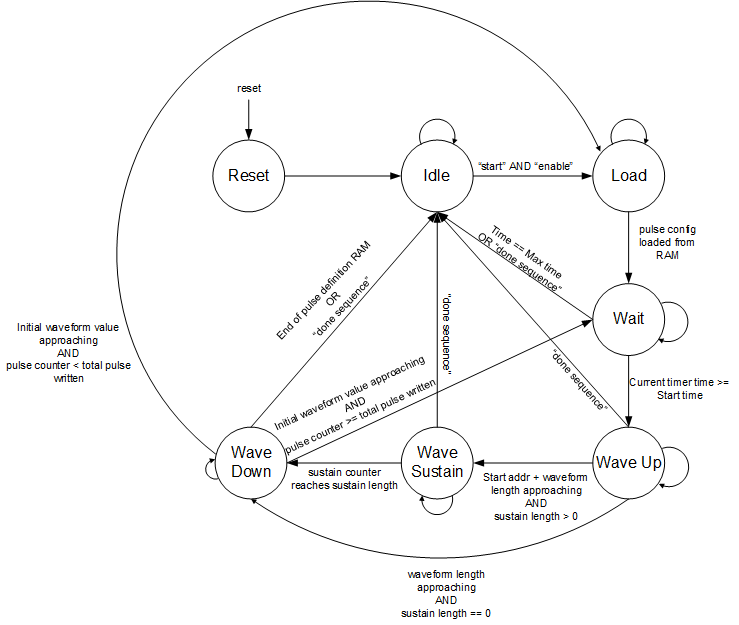
\includegraphics[width=1\linewidth]{figures/3.4.png}
    \caption{State Diagram of the Pulse Channel Module}
    \label{fig:fsm}
\end{figure}
When the timer reaches the start time, the module moves sequentially through the rise, sustain, and fall stages. During these stages, it carefully shapes the pulse by controlling both the waveform table address and its data output using the time and gain factor values. After the fall stage, the module evaluates whether additional pulses remain in the pulse definition memory. If there are more pulses, it immediately loads the next one. Otherwise, it waits for a "done sequence" signal before going idle.

An internal pulse counter monitors the current entry in the pulse definition memory and increments each time a new pulse is loaded. Because each pulse definition spans four memory addresses, the counter increases by four with every update. Another counter tracks the number of clock cycles that the sustain phase has lasted following the rise stage. When this counter reaches the defined sustain length, the state machine transitions to the fall stage. This organized, stage-based design simplifies the control logic while enhancing timing precision and signal integrity. 

In parallel, a separate process manages memory read and write operations via the CPU interface, indicated by the green arrows in \autoref{fig:block_diagram}. The pulse channel module extracts the lower 12 bits from the system address for either pulse definition memory or the waveform table memory. The 12th bit acts as a selection signal, effectively multiplexing data and addresses between these two memories. For the waveform table, each operation transfers a 32-bit value pair, which together constitute one entry. This arrangement yields a total of 2048 available entries for CPU accesses. In contrast, each pulse definition entry spans four 32-bit words. Therefore, it takes four consecutive CPU operations to complete one pulse definition entry. This clear division of memory operations not only ensures efficient and reliable data transfer but also simplifies the addressing scheme, maintaining data integrity and responsiveness in real-time FPGA applications.

\section{Error Handling}

The pulse channel is engineered to be highly robust and resilient, capable of handling both typical user inputs and unusual or invalid parameters. It accounts for common values as well as edge cases that might otherwise disrupt system operation. While the software interface manages most user-induced errors, the built-in error registers and handling mechanisms serve as the final safeguard. This layered approach prevents hazardous inputs from causing system failures, ensuring that the design remains safe and reliable even under unexpected conditions.

To ensure robust performance, several potential cases must be carefully considered. The design guarantees that pulses begin only when the current time meets or exceeds their scheduled start. Special attention is given to the sustain length. For instance, if a pulse definition specifies a flat-top length of zero, the system immediately transitions to the fall stage. The module also keeps track of the total number of generated pulses using the internal pulse counter, which helps maintain proper sequence control. Moreover, if the start time of a subsequent pulse is earlier than that of the previous one, the pulse is omitted to preserve timing integrity.

Additionally, the design manages cases where the waveform start address and length exceed the 4096-entry capacity of the waveform table memory. In such instances, the system either wraps the addresses correctly back into the valid range or triggers an error flag in an 8-bit register, with each bit defined in \autoref{table:erro_regs}. One-hot encoding ensures that the error register uniquely represents each error condition with a single active flag. When a specific error occurs, the system sets only the corresponding flag. This clear mapping simplifies fault diagnosis and reduces ambiguity during troubleshooting. When an error is detected, the system stops waveform generation to prevent the further propagation of invalid data, thereby maintaining overall system integrity. Furthermore, the registers are designed to log and maintain these error events, aiding in prompt debugging and corrective measures. The error registers can be cleared with an external clear flag or by resetting the system. Some registers have no error details assigned yet, allowing for future expandability based on further testing results.
\begin{table}[h]
\setlength{\abovecaptionskip}{5pt}    % Reduces space above caption
\setlength{\belowcaptionskip}{5pt}    % Reduces space below caption
\centering
\caption{Error Registers}
\label{table:erro_regs}
\begin{tabular}{|c|l|}
\hline
Register Bit & Error Details \\
\hline
0 & Wave table RAM overflow \\
\hline
1 & Rise length size $\leq$ 1 (need to min. 2) \\
\hline
2 & Time step bigger than the size of the rise \\
\hline
3 & Amplitude scale $>$ 1 \\
\hline
4 & Time step $<$ 1 \\
\hline
5 & \textit{Not yet assigned} \\
\hline
6 & \textit{Not yet assigned} \\
\hline
7 & \textit{Not yet assigned} \\
\hline
\end{tabular}
\end{table}
\chapter{Metrics For Evalutation}

This section outlines a comprehensive test plan for the pulse channel module, designed to rigorously evaluate its functionality, performance, and error-handling capabilities. The test strategy is systematically divided into distinct phases. Initially, it focuses on controlled experiments using predefined pulse sequences, ensuring that the module writes and reads fixed parameters accurately and that the hardware faithfully produces the expected pulse patterns. Next, the plan expands to include tests with randomly generated pulse parameters, simulating real-world conditions and assessing the design's robustness against unpredictable inputs. Finally, we validate the module's error detection mechanisms by deliberately injecting invalid parameters, confirming that the associated error flag registers correctly identify and report faults. Together, these testing stages build confidence in the module's reliability and performance, ensuring it meets the stringent requirements of advanced digital systems.

\section{Memory Access}

One of the essential metrics to evaluate is the pulse channel block's ability to read from and write to both the pulse definition and waveform table memories. This functionality is crucial because it directly affects the pulse channel's overall functionality and reliability. By continuously monitoring this capability throughout various testing phases, one can identify potential issues early on. This early detection ensures that data processed within the module remains consistent and accurate. Adopting this proactive approach not only maintains system stability but also prevents data corruption, thereby enhancing the overall integrity and efficiency of the system.

\section{Write Known Pulse}

An essential step in verifying the functionality of the pulse channel module is to perform a preliminary test using two to three predetermined pulses with fixed parameters. This carefully controlled test is designed to evaluate whether the hardware can accurately receive and produce known values, ensuring that each pulse is generated exactly as specified. Moreover, this initial validation helps identify potential issues before the module is deployed in scenarios involving more complex or real-world signal patterns. It provides a clear benchmark for performance, aids in troubleshooting early-stage design flaws, and supports iterative refinement of the system. In doing so, the test not only ensures compliance with the required technical specifications but also instills confidence in the module's ability to operate reliably under varying conditions. Overall, this methodical approach to testing reinforces the robustness of the hardware design, which is essential for both academic exploration and practical applications in advanced digital systems.

\section{Controlled Randomized Test}

After verifying that the hardware behaves as expected during initial tests—specifically that memory read and write operations execute correctly—a more comprehensive evaluation is initiated. In this phase, a software generator creates random pulse parameters and base rise values applicable to both the hardware design and its floating-point software equivalent model. This randomized input methodology is essential because it simulates a wide range of real-world conditions, thereby enhancing the testing process in terms of efficiency, reliability, and overall robustness. By confronting the system with unexpected yet realistic scenarios, designers can assess whether the hardware consistently performs its intended functions under diverse circumstances.

A software model calculates a theoretical floating-point value for each randomly generated pulse. This expected value serves as the benchmark for subsequent comparisons. However, since FPGA hardware operates with integer-based addresses and data, all pulse parameter values are scaled and then rounded down (floored) to the nearest integer before being written to memory or interfaced with other peripherals, as depicted in \autoref{fig:block_diagram}. After the conversion, the pulse waveform produced by the hardware is compared against the modeled floating-point value. Naturally, some discrepancies may emerge due to the inherent rounding process. To quantify these differences, an error metric is computed as the absolute difference between the theoretical and actual values. Additionally, a delta value is determined by measuring the difference between sequential output values from the hardware, providing further insight into the system's behavior over time. This comprehensive approach not only validates the hardware's capacity to process and generate pulses accurately but also highlights areas that may require further refinement, ensuring that the system meets stringent performance and reliability standards in practical applications.

\section{Check Error}

The pulse channel module is equipped with error flag registers designed to detect and flag invalid pulse parameters. To confirm that these error detection mechanisms operate as intended, we conduct tests by introducing deliberately invalid parameter values into the system. For example, configuring a pulse with a rise length of 1 and a step value of 2 is expected to simultaneously trigger the error flags in registers 1 and 2, as detailed in \autoref{table:erro_regs}. Systematically verifying that the system accurately identifies and reports these errors ensures the pulse channel's capability to handle unforeseen or erroneous conditions effectively. Ultimately, this testing strategy not only reinforces the robustness of the error handling but also enhances the overall reliability and resilience of the hardware under various operating scenarios.
% TODO: should this be reduced?\
\chapter{System Integration}


\begin{figure}[h]
    \setlength{\abovecaptionskip}{5pt}    % Reduces space above caption
    \setlength{\belowcaptionskip}{5pt}    % Reduces space below caption
    \centering
    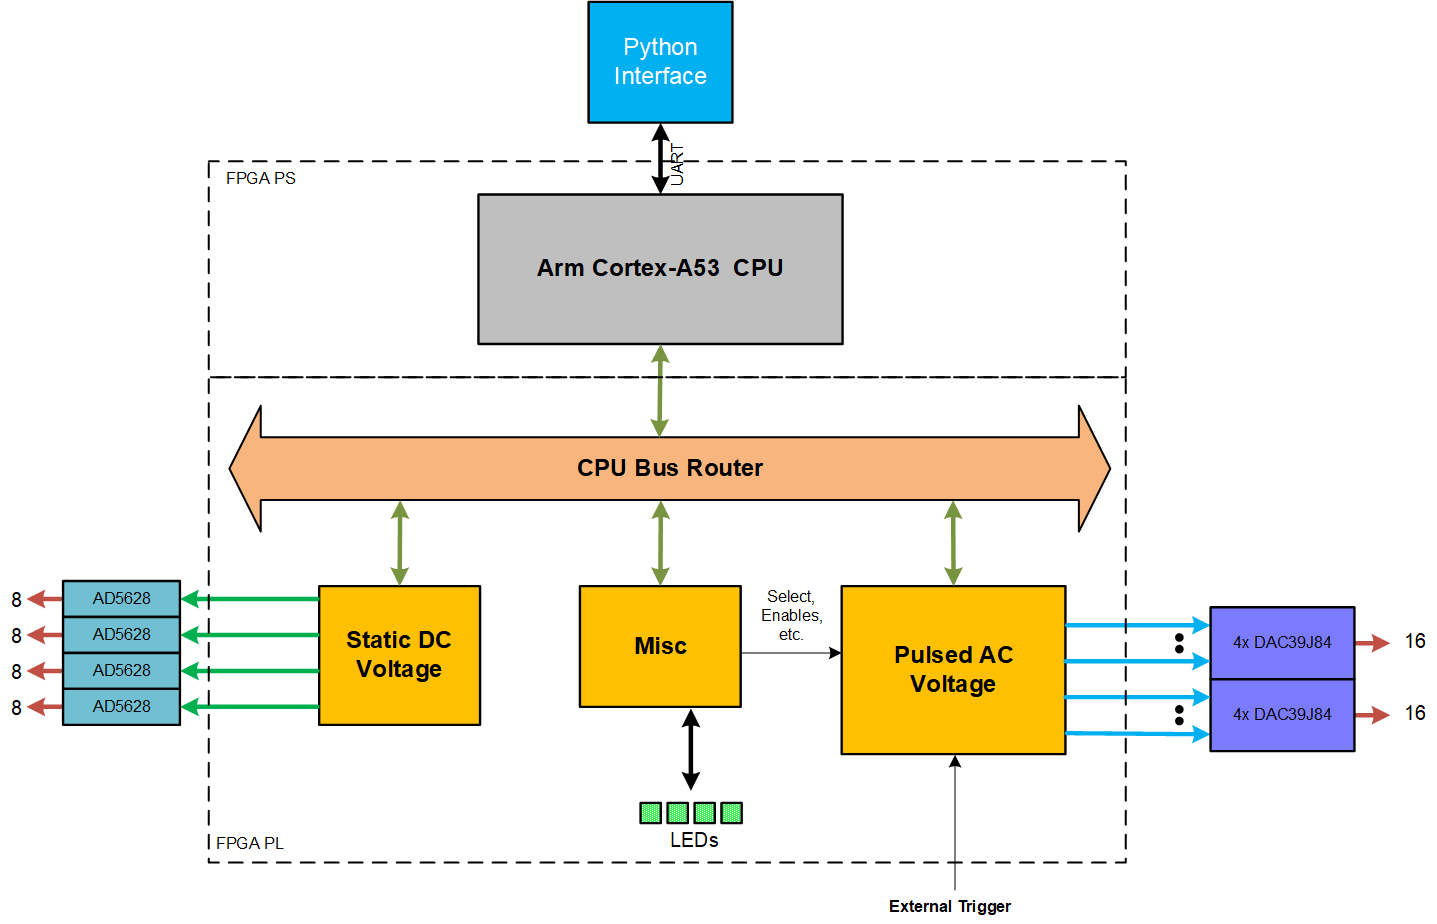
\includegraphics[width=1\linewidth]{figures/5.1.png}
    \caption{FPGA system architecture block diagram.}
    \label{fig:sys_diagram}
\end{figure}

The pulse channel module is an integral component of an FPGA system designed to generate 32 pulsed AC voltage signals and 32 static voltage signals. This system leverages both the processing systems and the programmable logic of the ZCU102 architecture. A Python-based interface allows users to input specific information about the pulses and voltage signals. This interface translates user requests into custom commands, which are then sent to the processing system via the FPGA's UART interface.

The processing system's ARM-based CPU converts Python-generated commands into addressable instructions for the FPGA's blocks. Within the FPGA hardware, a bus router takes the byte-addressable data from the CPU and translates it into block-specific word-addressable data. The system comprises three distinct hardware blocks, each serving a separate function. The orange blocks in \autoref{fig:sys_diagram} illustrate the names of these blocks, which will be discussed in detail in the subsequent sections. This architecture ensures efficient communication and data processing within the FPGA system, enhancing its overall performance and reliability.

% % TODO: this section is more translate Geoff to UW... does it rly needed to be mentioned in the thesis?
% \section{CPU Bus Router}

% The system utilizes a CPU interface adapter to bridge between the PS and the PL. This adapter plays a crucial role by converting byte-addressed signals from the PS AXI bus into a 32-bit word-addressed bus, which is essential for the proper functioning of the blocks within the FPGA design. Illustrated in \autoref{table:ps_addr}, the portions of the PS address are decoded into block select to choose one of the three available blocks in the system. Once a block is selected, the lower bits of the address are used to either write to or read from the chosen block. This ensures precise and efficient communication between the PS and the selected block. Additionally, a standardized register interface is implemented in each block to provide consistent access for control and status monitoring, thereby enhancing the system's reliability and ease of use. By employing this CPU interface adapter, the system achieves seamless integration between the PS and PL, facilitating efficient data transfer and control across the FPGA design. This design choice not only simplifies the communication process but also ensures scalability and flexibility for future enhancements.

 
% % TODO: explain more on this
% \begin{table}
% \centering
% \caption{Address convert format}
% 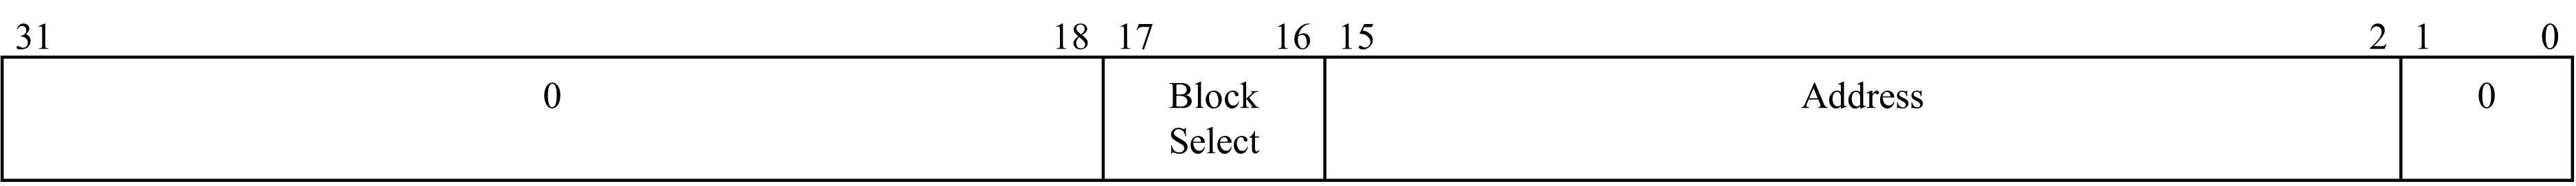
\includegraphics[width=1.0\textwidth]{figures/pc_address.png}
% \label{table:ps_addr}
% \end{table}

\section{Static DC Voltage Block}
% TODO: replace with a clear picture
\begin{figure}[h]
    \setlength{\abovecaptionskip}{5pt}    % Reduces space above caption
    \setlength{\belowcaptionskip}{5pt}    % Reduces space below caption
    \centering
    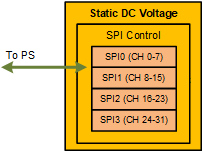
\includegraphics[width=0.5\linewidth]{figures/5.2.png}
    \caption{Block diagram for the DC voltage module}
    \label{fig:dc}
\end{figure}
The DC block provides stable and programmable static voltage control using four Analog Device AD5286 PMOD DACs. Each DAC supports eight voltage channels, making a total of 32 channels, as illustrated in \autoref{fig:dc}. Communication between the DACs and the system occurs via the SPI interface. These SPI interfaces are implemented as separate modules, each managing the clock, data, and chip select signals for data transmission to the DACs.

% TODO: Again... latex is not great for hardware so far...
\begin{table}[h]
\centering
\setlength{\abovecaptionskip}{5pt}    % Reduces space above caption
\setlength{\belowcaptionskip}{5pt}    % Reduces space below caption
\caption{SPI DAC message format}

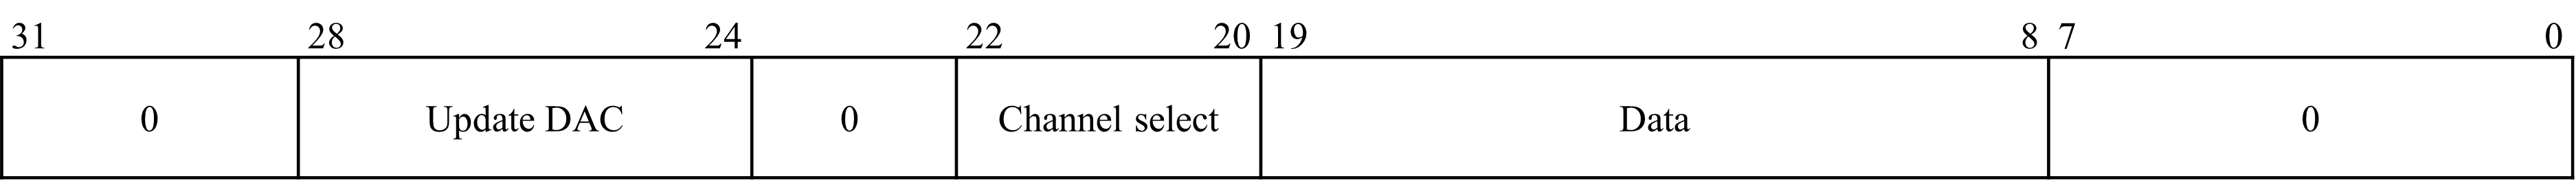
\includegraphics[width=1.0\textwidth]{figures/spi_addr.png}
\label{table:spi_addr}
\end{table}

% Upon selection, the DC block converts part of the address and the lower 12-bit data from the processing system into SPI command as defined in \autoref{table:spi_addr}. 
The DC block utilizes the lower five bits of the CPU address to select one of four SPI-based DACs. Part of the address is used in the SPI message for the chosen DAC, as detailed in \autoref{table:spi_addr}. This address segment specifies the "channel select" portion of the command, determining which of the eight channels on the selected DAC will be used. The SPI message also includes an "update DAC" command to instruct the DAC to refresh the chosen channel's value, which is set in the "data" portion of the message. The processing system provides a 12-bit positive integer value for the DACs, which is then converted to a voltage value as specified by:

\begin{equation}
V_{out} = V_{ref} \times \frac{D}{2^{12}}
\end{equation}

Where $V_{out}$ is the voltage output by the DAC, $V_{ref}$ is the DAC's reference voltage, and $D$ is the data from the processing system \cite{ad5628}. This design ensures precise and flexible static voltage control. Additionally, the module supports write operations to update DAC channels and control features such as internal reference voltage and power. It also supports read operations, which return status flags for each SPI transaction. The use of multiple DACs and independent SPI modules allows for efficient handling of numerous voltage channels, providing enhanced control and reliability.

\section{Pulse AC Voltage Block}

The pulse generation module—also referred to as the AC block—is a synchronous multi-channel pulse generator designed to deliver precise control for laser operations on the photonic chips. Its architecture generates pulse sequences with a 10-nanosecond resolution across 32 channels, ensuring that each digital output is synchronized. 

\begin{figure}[h]
    \setlength{\abovecaptionskip}{5pt}    % Reduces space above caption
    \setlength{\belowcaptionskip}{5pt}    % Reduces space below caption
    \centering
    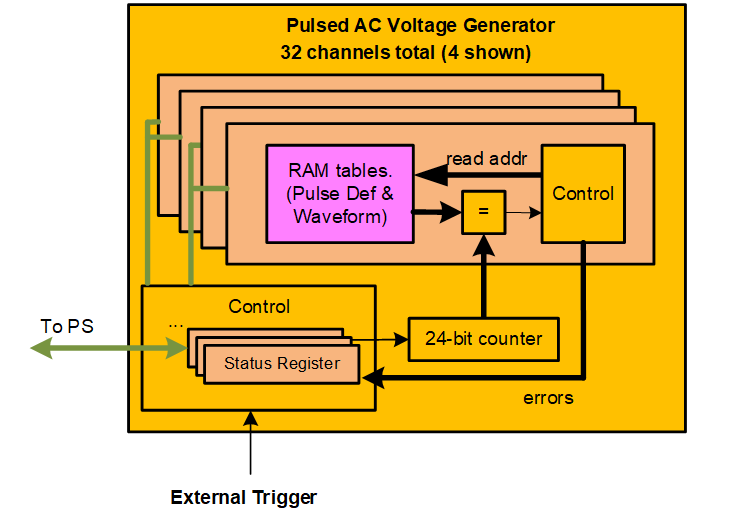
\includegraphics[width=0.8\linewidth]{figures/5.3.png}
    \caption{Block Diagram of the AC block.}
    \label{fig:george}
\end{figure}
The AC block acts as the central coordinator for all pulse channels. A Central Coordinator Process (CC-P) manages both external control signals and error notifications from individual channels, ensuring reliable overall performance. Central to its operation is a 24-bit counter that functions as a common timer, as seen in \autoref{fig:george}. Upon receiving an external trigger, this counter initiates the timing process uniformly for all channels. It continues until it reaches either a user-defined sequence length or its maximum value, at which point it sends stop signals to halt pulse generation. This coordinated stopping mechanism maintains timing precision and prevents runaway pulses that could lead to data inconsistencies.

A series of internal registers underpin the module's functionality. These registers store key parameters such as the total sequence length, the active channel enable, and select for memory reading and writing operations. Values are loaded into these registers via the CPU interface, which streams configuration data from the processing system. The design supports simultaneous writing to multiple channels, a useful feature for updating pulse parameters in parallel. However, because the data bus is only 32 bits wide, the system limits read operations to one channel at a time.

The module also incorporates an addressing scheme that distinguishes between channel-specific memory and internal control registers. The lower address range is reserved for waveform data and pulse parameters, while the upper range is dedicated to registers for the CC-P. Registers for settings such as sequence length, channel enables, and channel selections are both readable and writable. This bidirectional access permits real-time control and monitoring of each channel, facilitating adjustments as operational conditions change. In contrast, dedicated read-only registers continuously convey status information from both the module and the individual pulse channels.

Error handling within the AC block is equally streamlined. As discussed, each pulse channel generates error signals that are collected as multi-bit vectors. The CC-P then transposes these into several 32-bit registers, with each register corresponding to a specific error type defined in \autoref{table:erro_regs}. Within a given register, each bit represents the status of one of the 32 channels. This systematic condensation of error information into a single-dimensional format simplifies monitoring and debugging processes, enabling engineers to quickly identify and address issues.

\section{Miscellaneous}

The miscellaneous block is a versatile control and status interface integrated into the system. It manages a variety of auxiliary functions that streamline control processes. This module organizes basic operations, such as managing system interfacing, monitoring status, and distributing control signals. Its primary role is to bridge CPU control with hardware functionality through several dedicated registers. These registers handle tasks such as version reporting, LED indication, and debug routing. A notable feature is its configurable LED control system. This system allows either PS or PL to drive status indicators based on the LED enable register settings, providing flexibility and accurate control. Isolating these auxiliary functions enhances maintainability, simplifies debugging, and promotes reusability. Beyond its fundamental capabilities, the miscellaneous block streamlines operations and supports a modular system architecture.

\section{Software Control Interface}
% TODO: change this section to match the actual python once it has been re-made
A dedicated Python package translates user-defined waveform values and pulse information into addresses and data formats for the hardware. This abstraction bridges the gap between users with limited hardware design experience and the intricate nature of FPGA architectures. By automating tasks such as memory management and data formatting, the system enables users to focus on refining their quantum control strategies rather than wrestling with hardware-level operations. This design philosophy enhances both usability and performance across the entire framework.

The interface functions similarly to a streamlined web API, allowing users to submit waveform data and parameters intuitively. For every pulse entry, the software automatically locates the next available memory space, computes the starting address and length, and allocates the data accordingly, returning a unique waveform ID for straightforward reference. This methodical allocation ensures that inputs accumulate properly and that any error due to exceeding available memory is promptly flagged. Additionally, the system archives each waveform record in a dedicated file, providing traceability as detailed in \autoref{table:param_rec_table}. The first row for each column in the table represents a unique six-digit wave ID. The remaining rows are values for each waveform.

% TODO: add label to explain things
\begin{table}[h]
\setlength{\abovecaptionskip}{5pt}    % Reduces space above caption
\setlength{\belowcaptionskip}{5pt}    % Reduces space below caption
\centering
\caption{Sample Format of the Waveform Record}
\label{table:param_rec_table}
\begin{tabular}{|c|c|c|c|}
\hline
\textbf{Wave ID} & 262144 & 196612 & 327688\\
\hline
\multirow{5}{*}{\rotatebox[origin=c]{90}{\textbf{Waveform Values}}}%
&0 & 0 & 0 \\
\cline{2-4}
&1 & 2 & 5 \\
\cline{2-4}
&3 & 5 & 6\\
\cline{2-4}
&4 & - & 8\\
\cline{2-4}
& - & - & 12\\
\hline
\end{tabular}
\end{table}

In a similar fashion, pulse parameter management is performed through dedicated functions that support both loading and retrieval. Unlike waveform data, which can vary in length and address, pulse parameters are stored in fixed groups of four values. Users provide key details such as the pulse's start time, time factor, gain factor, and sustain time, along with the relevant waveform ID. The interface then leverages this ID to fetch additional hardware parameters—such as the corresponding waveforms start address and length—converting the user inputs into a hardware-accepted format as outlined in \autoref{fig:pd}b. Corresponding records are then logged in a file following the format shown in \autoref{table:wave_rec_table}.

\begin{table}[h]
\setlength{\abovecaptionskip}{5pt}    % Reduces space above caption
\setlength{\belowcaptionskip}{5pt}    % Reduces space below caption
\centering
\caption{Sample Format of the Pulse Parameter Record}
\label{table:wave_rec_table}
\begin{tabular}{|c|c|c|c|c|}
\hline
Wave ID & Start Time & Scale Gain & Scale Address & Sustain \\
\hline
262144 & 5 & 0.98 & 1.2 & 5\\
\hline
196612 & 48 & 1.0 & 1.1 & 7\\
\hline
327688 & 100 & 1.0 & 1.0 & 0\\
\hline
\end{tabular}
\end{table}

After processing, the serial interface passes these hardware-ready values to a custom Python class that integrates them with subroutines designed for the FPGA. Communication with the embedded ARM CPU is maintained via a UART connection, with the third-party PYSerial package ensuring reliable data transfer. Commands transmitted by the Python class are interpreted by the PS to activate specific design blocks defined in \autoref{fig:sys_diagram}. This layered control strategy not only streamlines user interaction but also preserves the precision and high performance required by contemporary FPGA applications.
\chapter{Outcome and Result}

% TODO: rewrite to independent from the test plan (may removed)
\section{Simulation Result}
\begin{figure}[h]
    \centering
    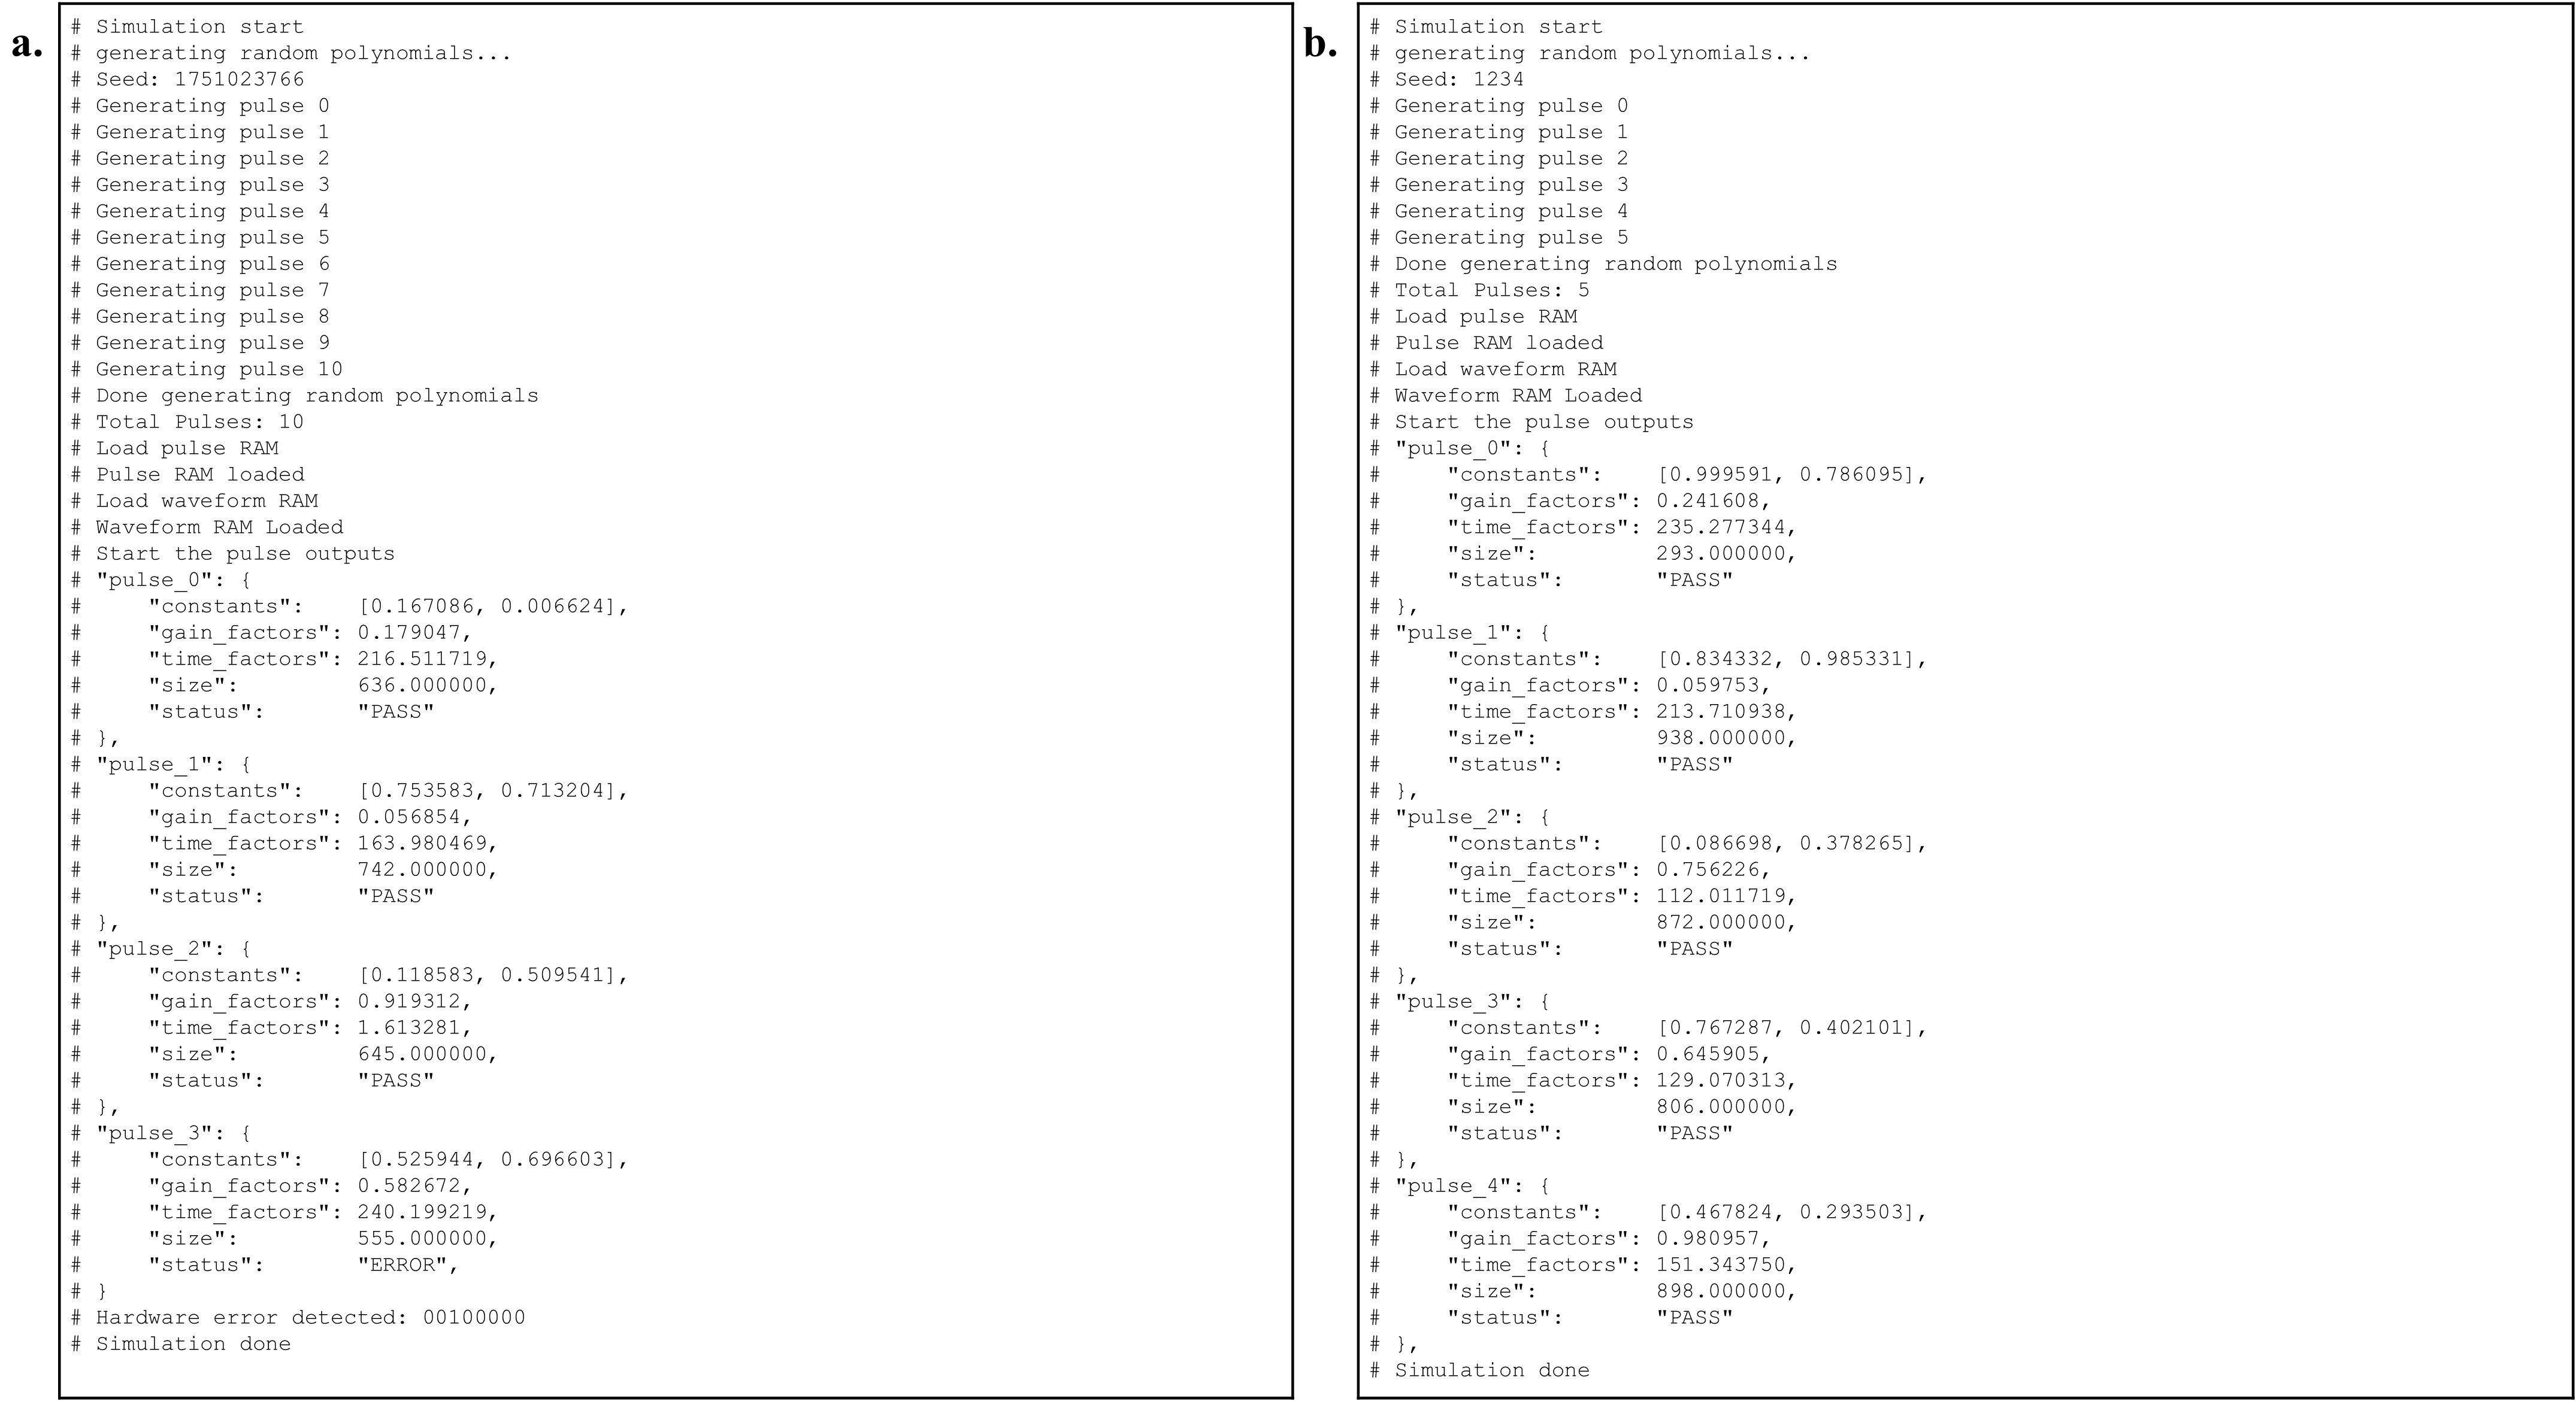
\includegraphics[width=1\linewidth]{figures/6.1.png}
    \caption{\centering{Simulation result of \textbf{a.} Seed with incorrect parameters and \textbf{b.} Seed with normal parameters}}
    \label{fig:6.1}
\end{figure}
To validate the functionality and ensure the reliability of the pulse channel module, a controlled randomized regression test was designed and implemented. This test serves as a comprehensive evaluation of the module’s performance across several key aspects. Specifically, it examines the module's ability to execute memory read and write operations efficiently, preserve data accuracy during these processes, and manage potential errors effectively.These assessments are the cornerstone of identifying and resolving any latent issues that could compromise the module's functionality in practical applications. The results of this testing process provide significant insights into the module's behavior and confirm its expected performance. \autoref{fig:6.1} illustrates two simulation outcomes, both generated using Intel ModelSim, which visually validate the module’s operation under the given test scenarios.

% A key component of this test is the use of a seed value to manage the randomization process. This seed, which begins at one and increments sequentially by one with each iteration, introduces controlled variability into the test inputs. The randomization ensures that the module's memories are subjected to diverse data patterns. These values are simultaneously applied to the module's memory system and a corresponding software model, which serves as a theoretical benchmark. By comparing the module's output with the software model, the hardware's accuracy is rigorously verified.

% \autoref{table:error_results} offers an illustrative snapshot of the first ten iterations of the regression test, outlining several key performance metrics. The column labeled "Seed" denotes the specific randomization seed used during each test, providing insight into the exact conditions under which the test was conducted. The "Time" metric indicates the elapsed duration from when a pulse is triggered to when the corresponding error is detected. Additionally, the "Error/Delta" value represents the ratio between the observed error and the reference delta, offering a quantitative measure of performance discrepancies. It is calculated by
% \begin{equation}
% \frac{Error}{Delta} = \frac{|\text{theoretical value} - \text{actual value}|}{|\text{current hardware output} - \text{previous hardware output}|}
% \end{equation}
% Finally, the "Pulse Number" specifies the sequential order of the pulse that produced the largest error-to-delta ratio during that iteration. Together, these detailed metrics enable us to thoroughly assess how the module responds under a wide spectrum of conditions, ultimately affirming its reliability and adherence to our stringent performance criteria.

% \begin{table}[h]
% \centering
% \caption{Simulation results for first 10 seeds}
% \begin{tabular}{|c|c|c|c|}
% \hline
% Seed & Time (ns) & Error/Delta & Pulse Number \\
% \hline
% 1 & 159490 & 0.0035 & 3 \\
% 2 & 175960 & 0.1932 & 4 \\
% 3 & 189310 & 0.0096 & 5 \\
% 4 & 156640 & 0.0149 & 2 \\
% 5 & 159900 & 0.0022 & 2 \\
% 6 & 159090 & 0.3055 & 3 \\
% 7 & 161220 & 0.2224 & 3 \\
% 8 & 163910 & 0.1640 & 3 \\
% 9 & 134220 & 0.0164 & 0 \\
% 10 & 134220 & 0.0302 & 0 \\
% \hline
% \end{tabular}
% \label{table:error_results}
% \end{table}


\section{Board Result}
The system is examined using Xilinx's Integrated Logic Analyzer (ILA) to validate signals from multiple modules, including the single pulse channel module.  
\begin{figure}[h]
    \centering
    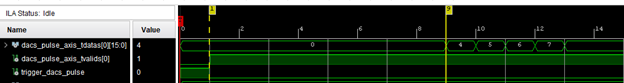
\includegraphics[width=1\linewidth]{figures/ila.png}
    \caption{ILA monitored the result from the top level.}
    \label{fig:ila}
\end{figure}

A 55-sample waveform, starting from a nonzero value at 50 ns, is transmitted to the hardware and captured by the ILA (see \autoref{fig:ila}). The first output appears after 8 cycles, with each cycle lasting 10 nanoseconds. This timing results in an 80-nanosecond delay, confirming that the pulse generation operates well within the sub-microsecond range required for quantum control hardware. Furthermore, ILA data indicate that data updates occur every 10 nanoseconds, highlighting the rapid switching performance required for high-speed applications. Additionally, an external oscilloscope recorded a pulse sequence in \autoref{fig:osc}, further verifying the overall functionality and behavior of the design.
\begin{figure}[h]
    \centering
    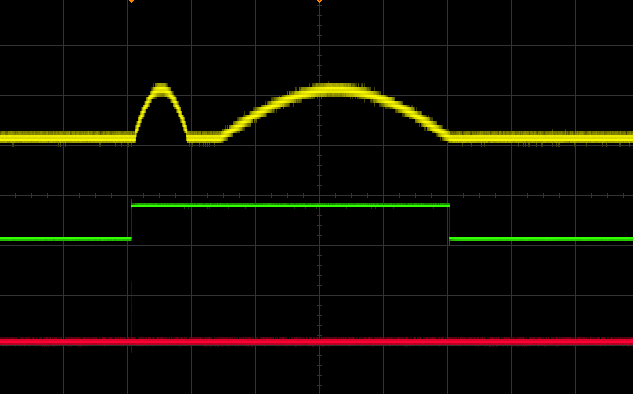
\includegraphics[width=.85\linewidth]{figures/one_trig_seq.png}
    \caption{\centering{A single pulse sequence captured on an oscilloscope. The yellow line is the pulse sequence, the green line is the valid signal, and the red line is the trigger signal.}}
    \label{fig:osc}
\end{figure}
% The ILA plays a 

\section{Resource Utilization}

In FPGA design, efficient resource utilization is integral for ensuring a high-quality, reliable system. One of the most core aspects of this evaluation is timing analysis. After implementation, the Xilinx Vivado tool generates an in-depth timing report that details the minimum and maximum delay paths within the design. Generated reports in \autoref{fig:sta} confirm that both setup and hold times meet the specified constraints.
\begin{figure}[ht]
    \centering
    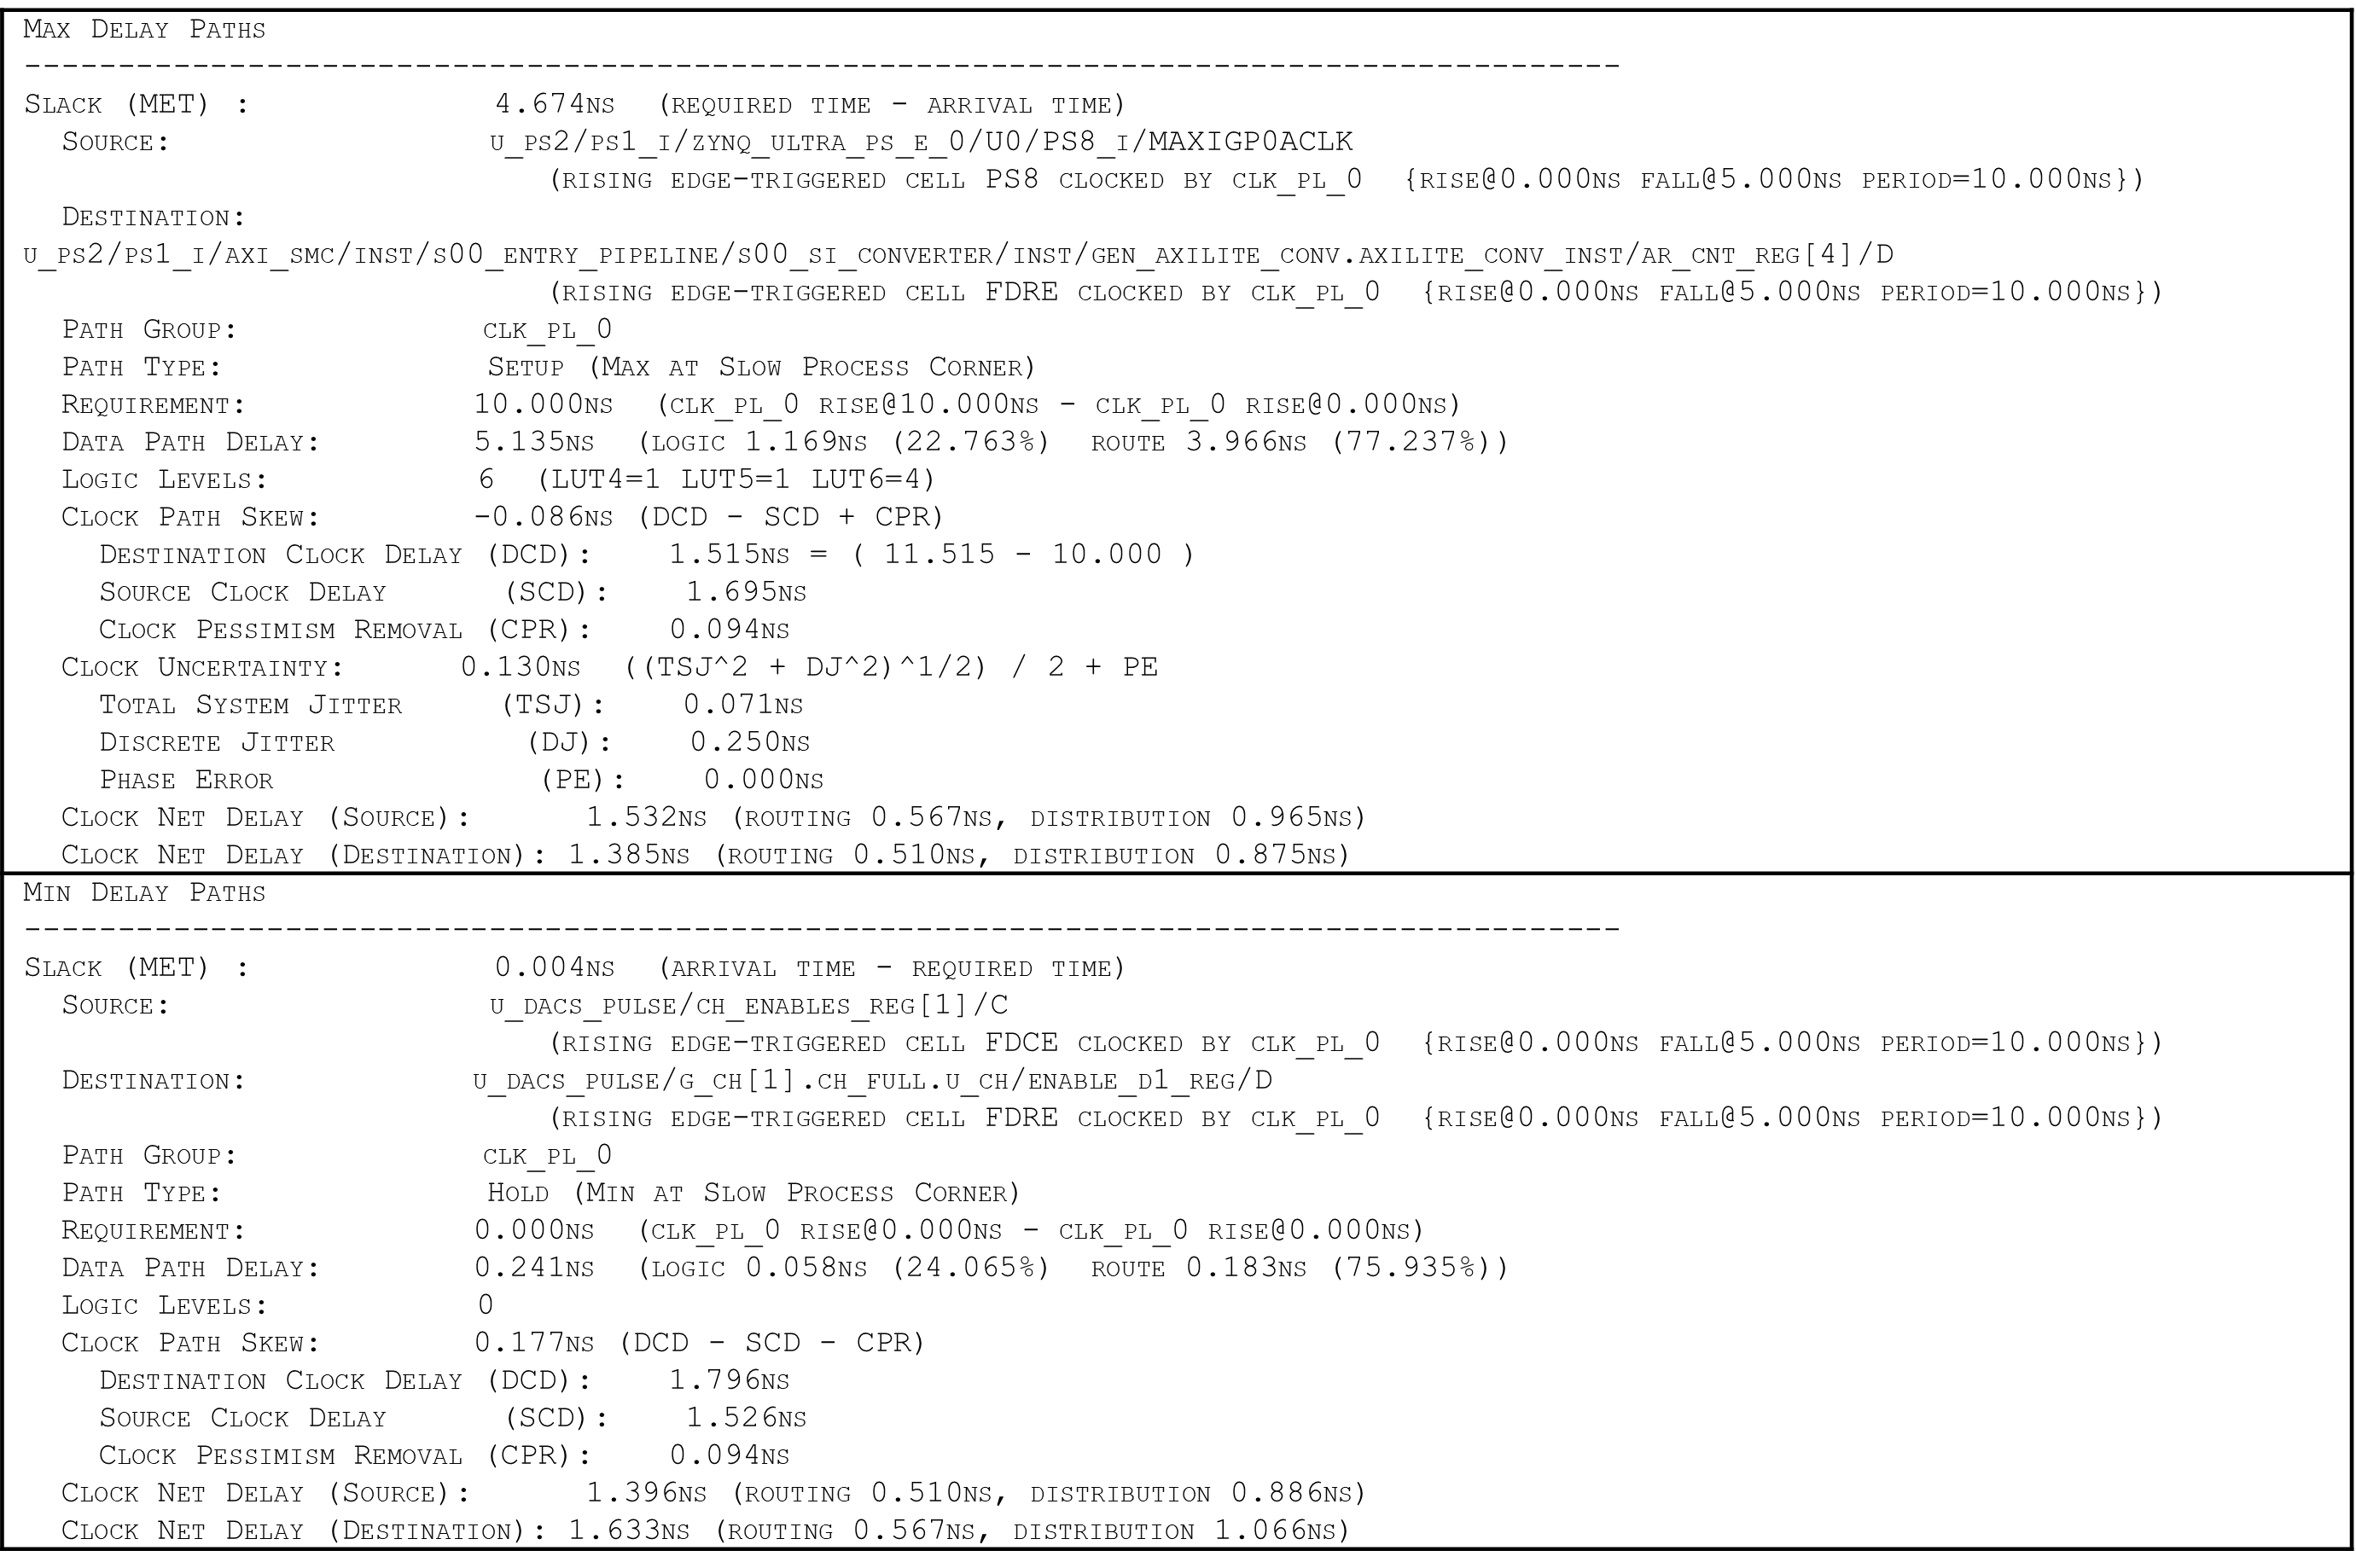
\includegraphics[width=1\linewidth]{figures/timimg_report.png}
    \caption{Partial timing report from Vivado on the worst slack (top) and hold (bottom).}
    \label{fig:sta}
\end{figure}
This timing verification ensures that all synchronous elements operate correctly within the designated clock cycle, preventing data corruption and operational failures. 

\autoref{table:chip_utilization} shows that only a small fraction of the FPGA resources are used. This low usage proves the design's efficiency. Minimal resource usage reduces power consumption. It also helps the FPGA maintain optimal timing and routing. This efficiency is ideal for scalable systems that may need future modifications. It validates the careful design decisions made during synthesis and optimization.

\begin{table}[ht]
\centering
\caption{Post-Implementation Resource Utilization Reported by Vivado}
\begin{tabular}{|l|r|r|r|r|}
\hline
On-Chip & Power (W) & Used & Available & Utilization (\%) \\ \hline
Clocks                  & 0.034   & 3     & ---    & ---      \\ \hline
CLB Logic               & 0.018   & 30403 & ---    & ---      \\ \hline
\quad LUT as Logic      & 0.015   & 12671 & 274080 & 4.62     \\ \hline
\quad CARRY8            & 0.002   & 909   & 34260  & 2.65     \\ \hline
\quad Register          & $<$0.001& 12952 & 548160 & 2.36     \\ \hline
\quad LUT as Shift Register & $<$0.001 & 4   & 144000 & $<$0.01 \\ \hline
\quad Others            & 0.000   & 567   & ---    & ---      \\ \hline
Signals                 & 0.029   & 24867 & ---    & ---      \\ \hline
Block RAM               & 0.174   & 128   & 912    & 14.04    \\ \hline
DSPs                    & $<$0.001& 2     & 2520   & 0.08     \\ \hline
I/O                     & 0.014   & 36    & 328    & 10.98    \\ \hline
PS8                     & 2.472   & 1     & ---    & ---      \\ \hline
Static Power            & 0.750   &       &        &          \\ \hline
\quad PS Static         & 0.098   &       &        &          \\ \hline
\quad PL Static         & 0.653   &       &        &          \\ \hline
Total                   & 3.492   &       &        &          \\ \hline
\end{tabular}
\label{table:chip_utilization}
\end{table}

\chapter{Discussion}

\section{Hardware Precision}

The current FPGA-based control system for quantum laser control demonstrates proof-of-concept functionality and lays a foundation for future applications. However, test results reveal consistent discrepancies between theoretical and measured values. These errors stem primarily from the rounding mechanism. \autoref{fig:block_diagram} indicates that data and address inputs in the waveform table memory are floored to the nearest integer, which discards important fractional components and limits resolution.

Waveforms are generated from predefined tables that are externally computed and then loaded into the system. This method simplifies on-chip logic and resource management by avoiding complex dynamic computations. However, using a fixed 16-bit integer representation introduces quantization errors when multiple write operations produce a complete waveform. The resulting trade-off between simplicity and precision underscores the limitations of the current design. To improve accuracy, enhanced rounding methods, such as midpoint rounding or adaptive precision schemes, could reduce truncation errors. Adopting dynamic waveform generation lowers the data transfer volume. In this approach, only key parameters—amplitude, frequency, and phase—are specified. The system computes the complete waveform in real time. This method produces waveforms that more closely match their theoretical definitions. The reduced data transfer volume also lowers storage and communication overhead.

\section{Hardware Error Handling}

The system utilizes a basic error detection framework that effectively identifies invalid parameters from the user. When an error occurs, the system sets a status flag for the controlling processor to read. However, it relies on a passive notification system rather than active error recovery. This approach depends entirely on a dedicated software interface to resolve issues, which can lead to complications if the software is not properly implemented or if user parameter conversions fail.

The pulse channel's definition memory assumes waveform parameters are provided in a consecutive, incrementing order. The hardware lacks a built-in mechanism to verify or correct this order. The module directly maps the provided address to the memory, which can lead to data inconsistencies if users do not sequence their parameters correctly. Future development should introduce a hardware mechanism to enforce cumulative writes of pulse parameters.

Additionally, permitting users to write to any memory location enhances system flexibility but also introduces the risk of overlapping writes. Without rigorous external software control over memory address management, the probability of data overwrites increases. Addressing this vulnerability in future work at the hardware level helps to maintain system stability and reliability.

% Subjected for removal if alternate firmware implemented
\section{Interface Latency}
% TODO: this is only the idea for new implementation... will get modified a lot after the new interface is done
Many user-level interfaces are implemented in Python on a separate PC, requiring UART serial writes to the hardware system. Each write transmits only 8 bits of data from the host to the FPGA, resulting in limited throughput and extended read and write times. Tests show that reading and writing an entire waveform and one pulse configuration each take an average of three to four seconds. These delays become significant bottlenecks, especially when the system needs to access memories multiple times during operation.

To mitigate this issue, sophisticated C firmware could replace much of Python's functionality in the future. This firmware would reside on Xilinx's processing system, fully leveraging Zynq's high-speed AXI interface to accelerate data transfers. Instead of relying on Python functions to relay user parameters, the processing system would accept input directly from a command-line interface. Users could manually type parameters or design scripts to automate their entry.
\chapter{Conclusion}

In this thesis, a novel laser control system for trapped-ion quantum experiments is introduced and successfully tested, demonstrating a breakthrough design implemented on the Xilinx Zynq FPGA platform. The system integrates external digital-to-analog converters to achieve synchronous control over 32 laser channels with a minimum switching time of 10 ns for the precision required in quantum waveform generation. To ensure reliability and performance, a single pulse channel capable of generating the desired waveform is first developed and thoroughly evaluated. This prototype is then scaled to the full system through the incorporation of custom programmable logic blocks. These blocks deliver stable DC voltage control alongside high-frequency pulsed waveform generation, ensuring versatile and accurate signal manipulation that meets the stringent demands of quantum experiments. By leveraging the FPGA's built-in features, the design attains both high performance and throughput. This strategic resource utilization guarantees precise hardware timing and maximum efficiency, addressing the complex challenges of laser control in trapped-ion systems. Furthermore, a sophisticated user interface is developed to allow users to focus on designing experiments rather than managing low-level hardware configurations. Collectively, these integrated features enhance system responsiveness and scalability, setting the stage for future innovations in quantum computing hardware.

%
% ==========   Bibliography
%
\nocite{*}   % include everything in the uwthesis.bib file
\bibliographystyle{plain}
\bibliography{uwthesis}


\end{document}
